%%%%%%%%%%%%%%%%%%%%%%%%%%%%%%%%%%%%%%%%%%%%%%%%%%%%%%%%%%%%%%%%%%
%% Scribe Editors: 
%%    - Jimmy Lin <jimmy@utexas.edu>
%%    - Vutha Va <vutha.va@utexas.edu>
%%    - David Inouye <davidinouye@gmail.com>
%%%%%%%%%%%%%%%%%%%%%%%%%%%%%%%%%%%%%%%%%%%%%%%%%%%%%%%%%%%%%%%%%%
%% The main content of LECTURE 07 contains THREE SECTIONS. 
%% Specifically,
%%    ONE: definition and interpretations of Newton step
%%    TWO: Affine Invariance of Newton step
%%    THREE: Convergence Analysis of Newton Method/step
%%%%%%%%%%%%%%%%%%%%%%%%%%%%%%%%%%%%%%%%%%%%%%%%%%%%%%%%%%%%%%%%%%
%% Copyright (c), JIMMY, VUTHA, DAVID @ UT AUSTIN 2014
%%%%%%%%%%%%%%%%%%%%%%%%%%%%%%%%%%%%%%%%%%%%%%%%%%%%%%%%%%%%%%%%%%
\documentclass{beamer}
\usepackage{mathptmx,wrapfig}
%\usepackage{helvet}
\mode<presentation>
{
  \usecolortheme{rose}
  \usecolortheme{dolphin}
  \setbeamercolor*{author in head/foot}{parent=palette secondary}
  \setbeamercolor*{title in head/foot}{parent=palette tertiary}
  \useinnertheme{rectangles}
  \setbeamertemplate{navigation symbols}{}
  \setbeamertemplate{footline}{
  \leavevmode%
  \hbox{%
  \begin{beamercolorbox}[wd=.5\paperwidth,ht=2.25ex,dp=1ex,center]{author in head/foot}%
    \usebeamerfont{author in head/foot}\insertshortauthor~~\insertshortinstitute
  \end{beamercolorbox}%
  \begin{beamercolorbox}[wd=.5\paperwidth,ht=2.25ex,dp=1ex,center]{title in head/foot}%
    \usebeamerfont{title in head/foot}\insertshorttitle
  \end{beamercolorbox}}%
  \vskip0pt%
  }
  \setbeamertemplate{frametitle}[default][center]
}
\usepackage[english]{babel}
\usepackage{epsfig}
\usepackage{hyperref}
\usepackage{graphicx}
\usepackage{amsthm}
\usepackage{amsmath}
\usepackage{amsfonts}
\usepackage{amssymb}
\usepackage{listings}
%\input{psfig.sty}
\newcommand{\ip}[2]{\langle #1,#2 \rangle}
\newtheorem{result}{Result}
%%%%%%%%%%%%%%%%%%%%%%%%%%%%%%%%%%%%%%%%%%%%%%%%%%%%%%%%%%%%
%%% Macros and setting outside the template
%%%%%%%%%%%%%%%%%%%%%%%%%%%%%%%%%%%%%%%%%%%%%%%%%%%%%%%%%%%%
\DeclareMathOperator{\dom}{dom}
\setbeamertemplate{caption}[numbered]
%%%%%%%%%%%%%%%%%%%%%%%%%%%%%%%%%%%%%%%%%%%%%%%%%%%%%%%%%%%%
%%% Document informatics
%%%%%%%%%%%%%%%%%%%%%%%%%%%%%%%%%%%%%%%%%%%%%%%%%%%%%%%%%%%%
\title{Large Scale Optimization: Lecture 7}
\author{Jimmy Lin, Vutha Va and David Inouye} 
\institute[]{The University of Texas at Austin} 
\date{September 23, 2014}
\begin{document}
%%%%%%%%%%%%%%%%%%%%%%%%%%%%%%%%%%%%%%%%%%%%%%%%%%%%%%%%%%%%
%% TITLE PAGE
%%%%%%%%%%%%%%%%%%%%%%%%%%%%%%%%%%%%%%%%%%%%%%%%%%%%%%%%%%%%
\begin{frame}
\titlepage
\end{frame}

%%%%%%%%%%%%%%%%%%%%%%%%%%%%%%%%%%%%%%%%%%%%%%%%%%%%%%%%%%%%
%% Section ONE: definition and interpretations of Newton Method
%%%%%%%%%%%%%%%%%%%%%%%%%%%%%%%%%%%%%%%%%%%%%%%%%%%%%%%%%%%%
\begin{frame}
\frametitle{Newton Step}
\begin{definition}
    For $x \in \dom f,$ the vector 
    \begin{align}
        \Delta x_{nt} = - \nabla^2 f(x)^{-1} \nabla f(x)
    \end{align}
    is called {\it Newton step} for function $f(\cdot)$ at point $x$. 
\end{definition}
\begin{itemize}
\item Note that $f(\cdot)$ is twice differentiable. 

\item Because $\nabla^2 f(x)$ is positive definite, 
    \begin{align}
        \nabla f(x)^T \Delta x_{nt} = -\nabla f(x)^T \nabla^2 f(x)^{-1} \nabla f(x) < 0
    \end{align}
unless $\nabla f(x) = 0$. So the Newton step is a descent direction unless $x$ is
already optimal.
\end{itemize}
\end{frame}
%%%%%%%%%%%%%%%%%%%%%%%%%%%%%%%%%%%%%%%%%%%%%%%%%%%%%%%%%%%%
\begin{frame}
\frametitle{Interpretation I}
\framesubtitle{Minimizer of second-order Approximation}
    Second-order Taylor approximation $\hat{f}$ of $f$ at $x$ is
    \begin{align}
    \hat{f}(x+v) = f(x) + \nabla f(x)^T v + \frac{1}{2} v^T \nabla^2 f(x) v
    \end{align}
    where RHS is minimized at direction
    \begin{align}
        v = - \nabla^2 f(x)^{-1} \nabla f(x) = \Delta x_{nt} 
    \end{align}
Combined with update rule, we have Newton update
    \begin{align}
    x^{+} = x - t \nabla^2 f(x)^{-1} \nabla f(x)
    \end{align}
    where $t$ is fixed step size.
\end{frame}
%%%%%%%%%%%%%%%%%%%%%%%%%%%%%%%%%%%%%%%%%%%%%%%%%%%%%%%%%%%%
\begin{frame}
\frametitle{Interpretation I}
\framesubtitle{Minimizer of second-order Approximation}
\begin{figure}
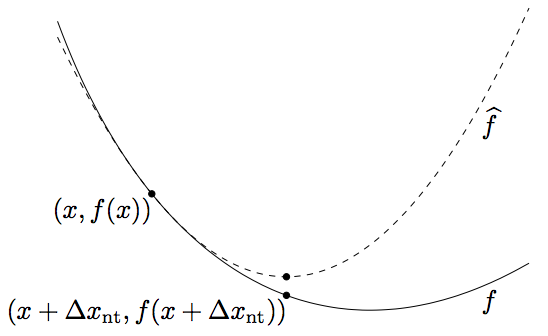
\includegraphics[width=2.2in]{minimizer.png}
\caption{
The function $f$ (shown solid) and its second-order approximation
$\hat{f}$ at $x$ (dashed). The Newton step $\Delta x_{nt}$ is what must be added to $x$ to give the minimizer of $\hat{f}$. [Figure and caption from  \textit{Convex Optimization} by Boyd and Vandenberghe.]
}
\label{fig:1}
%\footnote{ \tiny
%    Illustration and caption from \textit{Convex Optimization},  Boyd and Vandenberghe, 2004}
\end{figure}
\end{frame}
%%%%%%%%%%%%%%%%%%%%%%%%%%%%%%%%%%%%%%%%%%%%%%%%%%%%%%%%%%%%
\begin{frame}
\frametitle{Interpretation II}
\framesubtitle{Steepest descent direction in Hessian norm}
    Newton step can also be interpreted as 
    steepest descent direction when the norm is defined as
    \begin{align}
        \| u \|_{\nabla^2 f(x)} \triangleq \sqrt{u^T \nabla^2 f(x) u}
    \end{align}
    % XXX commented out by Vutha: This is rephrasing from the text, and I don't think we did anything about $||\cdot||_P$ norm, and the point given here is not easy to see from the given description either.
%    Recall from our discussion over steepest descent method that 
%    $ P = \nabla^2 f(x)$ is a very good choice as norm $||\cdot||_P$ inselecting
%    steepest descent direction, when $x$ is near $x^{*}$. Around $x^{*}$, we have $\nabla^2
%    f(x) \approx \nabla^2 f(x^{*})$, which explains why the Newton step is a
%    very good choice of search direction. See Figure \ref{fig:2}.
\end{frame}

\begin{frame}
\frametitle{Interpretation II}
\framesubtitle{Steepest descent direction in Hessian norm}
\begin{figure}
    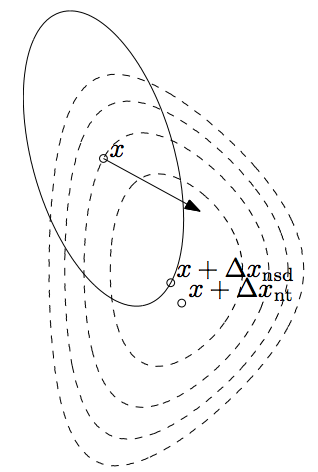
\includegraphics[width=1.2in]{steepest.png}
\caption{ \footnotesize
The dashed lines are level curves of a convex function. The ellipsoid shown
(with solid line) is $\{x + v | v^T \nabla^2 f(x) v \leq 1\}$. The arrow shows
$-\nabla f(x)$, the gradient descent direction. The Newton step $\Delta x_{nt}$ is the
steepest descent direction in the norm $\|\cdot \|_{\nabla^2 f(x)}$. [Figure and caption from  \textit{Convex Optimization} by Boyd and Vandenberghe.] 
} 
\label{fig:2}
%\footnote{ \tiny
%    Illustration and caption from \textit{Convex Optimization},  Boyd and Vandenberghe, 2004}
\end{figure}
\end{frame}
%%%%%%%%%%%%%%%%%%%%%%%%%%%%%%%%%%%%%%%%%%%%%%%%%%%%%%%%%%%%
\begin{frame}
\frametitle{Interpretation III}
\framesubtitle{Solution of linearized optimality condition}
    Newton step can also be interpreted as 
    linear approximation over gradient $\nabla f(x)$ around $x$.
    \begin{align}
        \nabla f(x+v) \approx \nabla f(x) + \nabla^2 f(x) v
    \end{align}
    Set RHS to zero gives Newton step $\Delta x_{nt}$
    \begin{align}
        v = - \nabla^2 f(x)^{-1} \nabla f(x) = \Delta x_{nt} 
    \end{align}
    %%% TODO: add more comment
    So the Newton step $\Delta x_{nt}$ is what must be added to $x$ so that
    the linearized optimality condition holds. 

    Again, this suggests that when $x$ is near $x^{\star}$, the update $x+\Delta
    x_{nt}$ should be a very good approximation of $x^{\star}$.
\end{frame}
\begin{frame}
\frametitle{Interpretation III}
\framesubtitle{Solution of linearized optimality condition}
\begin{figure}
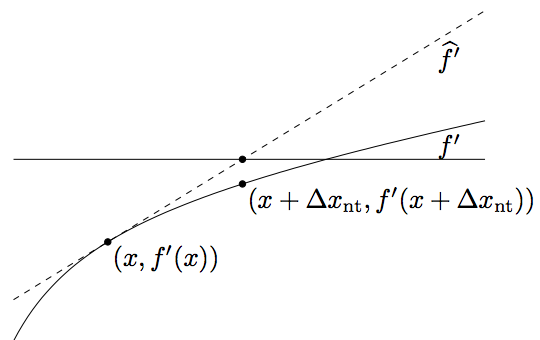
\includegraphics[width=2.5in]{linear.png}
\label{fig:3}
\caption{
The solid curve is the derivative $f'$ of the function $f$ shown in Figure
\ref{fig:2}.
$\hat{f'}$ is the linear approximation of $f'$ at $x$. The Newton step
$\Delta x_{nt}$ is the difference between the root of $\hat{f'}$ and the point $x$. [Figure and caption from  \textit{Convex Optimization} by Boyd and Vandenberghe.]
}
%\footnote{\tiny
%Illustration and caption from \textit{Convex Optimization},  Boyd and Vandenberghe, 2004}
\end{figure}
\end{frame}

%%%%%%%%%%%%%%%%%%%%%%%%%%%%%%%%%%%%%%%%%%%%%%%%%%%%%%%%%%%%
%% Section TWO: Affine Invariance of Newton step
%%%%%%%%%%%%%%%%%%%%%%%%%%%%%%%%%%%%%%%%%%%%%%%%%%%%%%%%%%%%
\begin{frame}
\frametitle{Affine Invariance of Newton step}
\begin{lemma}
    Newton step is affine invariant. 
\end{lemma}
For example, let $g(y) = f(Ay)$, $y^{+}$ be Newton update on function
$g(\cdot)$, and 
$x^{+}$ be Newton update on function $f(\cdot)$. 
Then if $x=Ay$, we have $x^{+} = Ay^{+}$.
\begin{block}{Remark}
    Affine Invariance indicates that Newton Method is invulnerable to the
    selection of coordinate system. 
\end{block}
\begin{block}{Remark}
    Gradient Descent Method is not affine invariant. This means
    that bad coordinate choice may limit the power of Gradient Descent Method.
\end{block}
\end{frame}
%%%%%%%%%%%%%%%%%%%%%%%%%%%%%%%%%%%%%%%%%%%%%%%%%%%%%%%%%%%%
\begin{frame}
\frametitle{Proof of Affine Invariance of Newton step}
    Let $x = Ay$ and $g(y) = f(Ay)$, then we have
    \begin{align}
       \nabla^2_{y}g(y) &= \nabla^2_{y}f(Ay) = A^T \nabla^2_{x}f(x) A \\
       \nabla_{y}g(y)   &= \nabla_{y}f(Ay) = A^T \nabla_{x}f(x)
    \end{align}
    Newton update $y^{+}$ for $g(\cdot)$ can be expanded as
    \begin{align}
        y^{+} &= y - t(\nabla^2_{y}g(y)^{-1} \nabla_{y}g(y)      \nonumber \\
        &= y - t(A^T \nabla^2_{x}f(x) A)^{-1} A^T \nabla_{x}f(x) \nonumber \\
        &= y - t\ A^{-1} \nabla^2_{x}f(x)^{-1} \nabla_{x}f(x)
    \end{align}
    Multiply both sides by $A$, 
    \begin{align}
        Ay^{+} &= Ay - A \cdot t\ A^{-1} \nabla^2_{x}f(x)^{-1} \nabla_{x}f(x)  \nonumber \\
        &= x - t\ \nabla^2_{x}f(x)^{-1} \nabla_{x}f(x) \nonumber \\
        &= x^{+}
    \end{align}
\end{frame}
%%%%%%%%%%%%%%%%%%%%%%%%%%%%%%%%%%%%%%%%%%%%%%%%%%%%%%%%%%%%
%% Section three: Newton Method
%%%%%%%%%%%%%%%%%%%%%%%%%%%%%%%%%%%%%%%%%%%%%%%%%%%%%%%%%%%%

%%%%%%%%%%%%%%%%%%%%%%%%%%%%%%%%%%%%%%%%%%%%%%%%%%%%%%%%%%%%
%% Section Four: Convergence Analysis of Newton Method
%%%%%%%%%%%%%%%%%%%%%%%%%%%%%%%%%%%%%%%%%%%%%%%%%%%%%%%%%%%%
\begin{frame}
    \frametitle{Convergence Analysis: Assumption}    
        %Let $f(\cdot)$ be the function discussed for Convergence of Newton Method. Both of following assumptions are what our convergence analysis relies on.
        We assume $f(\cdot)$ satisfies the following:
        \begin{itemize}
            \item $f(\cdot)$ is strongly convex, such that
    \begin{align}
        m I \preceq \nabla^2 f(x) \preceq M I, \hspace{0.5cm}\forall x
    \end{align}
\item $\nabla^2 f(x)$ is $L$-Lipschitz with constant $L > 0$, such that
    \begin{align}
        \| \nabla^2_{}f(y)  - \nabla^2_{}f(x) \|_2 \leq L \|x-y\|_2,\ 
        \forall x,\ y
    \end{align}
        Note that induced matrix norm $\| \cdot \|_2$ equals to the largest
        singluar value of the matrix.
        \end{itemize}
\end{frame}

%% theorem for each phase and implication by each phase
\begin{frame}
    \frametitle{Convergence Analysis: Theorem}    
    \begin{theorem}[Part I]
        There exist $\eta,\ \gamma$, where $ 0 < \eta \leq \frac{m^2}{L}$,
        $\gamma = \frac{\alpha \beta m}{M^2}\eta^2$
        such that Newton method with BTLS has two phases: 
        \begin{itemize}
            \item[(a)] Global or Damped Phase: If $\|\nabla f(x)\|_2 \geq \eta$, then 
                \begin{align}
                    f(x^{+}) - f(x) \leq -\gamma %, \text{ also } 
                    \label{CA:Theorem:phaseA}
                \end{align}
        \end{itemize}
    \end{theorem}
        Inequality \eqref{CA:Theorem:phaseA} has three implications: 
        \begin{itemize}
            \item Every Newton step with BTLS gets closer to global optima by
                at least $\gamma$.
            \item Damped phase has at most $\frac{f(x^{(0)}) -
                    f^{\star}}{\gamma}$ iterations.
            \item The damped phase is also at least linearly convergent if not better, i.e. $f(x^{+}) - f^\star \leq c(f(x)-f^\star)$
            
        \end{itemize}
\end{frame}

\begin{frame}
    \frametitle{Convergence Analysis: Theorem}    
    \begin{theorem}[Part II]
        \begin{itemize}
            \item[(b)] Local or Quadratic Phase: If $\|\nabla f(x)\|_2 < \eta$,
                then BTLS will give $t = 1$ and we have
                \begin{align}
                    \frac{L}{2m^2} \|\nabla_{}f(x^{+})\|_2 \leq 
                    \bigg(\frac{L}{2m^2} \|\nabla f(x)\|_2 \bigg)^2
                \end{align}
        \end{itemize}
    \end{theorem}
    Implication:
    \begin{itemize}
    \item To achieve an accuracy of $\epsilon$, only $O(\log \log \epsilon)$ iterations are needed once in the quadratic phase, which is known as quadratic convergence. [detail next slide]
    % XXX Commented out by Vutha: I think these points are redundant
    %\item Also, for strongly convex functions, $f(x) \to p^{*}$ quadratically.
    \end{itemize}
\end{frame}

\begin{frame}
	\frametitle{Implication of Part (b)}
	If we have $a_1 (<1), a_2,\dots$ such that $a_{i+1}\le a_{i}^2$, then
	\begin{align*}
	a_\ell \le (a_{\ell-1})^2 \le (a_{\ell-2})^{2^2} \le (a_{\ell-3})^{2^{3}} \le \dots \le (a_{1})^{2^{\ell-1}}
	\end{align*}
	for $a_\ell \le \epsilon$ need,
	\begin{align*}
	(a_{1})^{2^{\ell-1}} & \le \epsilon 
	\\  2^{\ell-1} \log a_1 & \le \log \epsilon
	\\   \ell  & \ge \log \log \frac{1}{\epsilon} + \text{constant}
	\end{align*}
	\begin{itemize}
	\item In this case to make it more precise, set $a_\ell = \frac{L}{2m^2} \|\nabla f(x^{(k+\ell - 1)}) \|_2$ and note that $a_1 < \frac{L}{2m^2}\eta < \frac{1}{2}$
	\end{itemize} 
\end{frame}

% TODO: proof of step size t = m/M satisfies the exit condition for BTLS
\begin{frame}
    \frametitle{Convergence Analysis: Part (a)}    
    %The way we prove convergence in global phase (a) is to employ a particular step size $t$, then show that this particular $t$ will eventually end the loops of BTLS and the desired inequal property holds under the exiting condition of BTLS. 
    For readability of the proof, we will divide the proof into lemmas. Use the following lemma for part (a).
    
    \begin{lemma}[Global BTLS]
        $t = \frac{m}{M}$ satisfies the exit condition of BTLS.
    \end{lemma}
    
    We will first prove the lemma and then the main result, which is 
    \begin{Theorem}[Part (a)]
        If $\|\nabla f(x)\|_2 \geq \eta$, 
        then $f(x^{+}) - f(x) \leq -\gamma$, 
        where  $\gamma = \frac{\alpha \beta m}{M^2}\eta^2$
    \end{Theorem}
    
    \begin{itemize}
    \item Notation: For convenience, $g\triangleq \nabla f(x)$ and $H\triangleq \nabla^2f(x)$
    \end{itemize}
    
\end{frame}

\begin{frame}
    \frametitle{Convergence Analysis: Part (a)}    
    \framesubtitle{Proof of Global BTLS Lemma}
    \begin{align}
        f(x^{+}) & = f(x-tH^{-1}g) \nonumber \\
        & \le f(x) - tg^TH^{-1}g + \frac{M}{2}t^2g^TH^{-1}H^{-1}g \label{froma} \\
        & \le f(x) - tg^TH^{-1}g + \frac{M}{2m}t^2 g^T H^{-1}g \label{tob}\\
        & = f(x) -  \frac{m}{2M} g^T H^{-1}g  &&
        \text{by setting $t=\frac{m}{M}$} \nonumber \\
        & \le f(x) - \alpha \frac{m}{M} g^T H^{-1}g && \text{since }\alpha <
        \frac{1}{2} \nonumber
    \end{align}
    %Note that\footnote{Recall the definition of square root of a matrix. If A is positive definite then we can write $A=U \Lambda U^T$, where $U$ is unitary and $\Lambda$ is diagonal, and $A^{1/2}=U \Lambda^{1/2} U^T$. },
Hence, $t = \frac{m}{M}$ satisfies the BTLS exit condition.

Note \eqref{froma} $\Rightarrow$ \eqref{tob} follows because,
\begin{align}
g^TH^{-1}H^{-1}g = g^TH^{-1/2}H^{-1}H^{-1/2}g \le \frac{1}{m} g^T H^{-1}g \nonumber
\end{align}
\end{frame}

% proof of inequality for (a) phase and show linear convergence inequality
\begin{frame}
    \frametitle{Convergence Analysis: Main Proof of Part (a)} 
%    \framesubtitle{Proof of Damped Phase Lemma}
	\begin{align}
	t &\leq \beta \frac{m}{M} \tag{Global BTLS Lemma} \\
	f(x^+) &\leq f(x) - \alpha\left(\beta \frac{m}{M} \right) g^T H^{-1} g \tag{BTLS condition} \\
	&\leq f(x) - \alpha\left(\beta \frac{m}{M} \right) \left(\frac{1}{M}\|g\|_2^2 \right) \tag{$H^{-1} \preceq I/m$} \\
	&= f(x) - \alpha\beta \frac{m}{M^2}\|g\|_2^2 \notag \\
	&\le f(x) - \underbrace{\alpha\beta \frac{m}{M^2} \eta^2}_{\gamma} \\
	&\implies f(x^+) - f(x) = - \gamma
	\end{align}
\end{frame}


%%%%%%%%%%%%%%%%%%%%%%%%%%%%%%%%%%%%%%%%%%%%%%%%%%%%%%%%
% proof of inequality for (b) phase
\begin{frame}
    \frametitle{Convergence Analysis: Part (b)}
    % XXX modified by Vutha: I think it's too wordy
%    Now cast our focus to provide the convergence guarantee when $\|\nablaf(x)\|_2 < \eta$ is the case. Similarly, we address the proof by dividing it into two separate lemmas.
	We will use the following lemma for this part.
    \begin{lemma}[Local BTLS]
        With the assumptions in (b), $t = 1$ satisfies the exit condition of BTLS.
    \end{lemma}
    Proof: See lecture note and text book.
    
    % Proof omitted because of space.  See p. 490-491 in Boyd.
    \begin{theorem}[Part (b)]
        If $\|\nabla f(x)\|_2 < \eta$, then 
        $ \frac{L}{2m^2} \|\nabla_{}f(x^{+})\|_2 \leq
                \bigg(\frac{L}{2m^2} \|\nabla f(x)\|_2 \bigg)^2 $
    \end{theorem}

\end{frame}
%%%%%%%%%%%%%%%%%%%%%%%%%%%%%%%%%%%%%%%%%%%%%%%%%%%%%%%%
\begin{frame}
    \frametitle{Convergence Analysis: Part (b)}
    %\framesubtitle{Proof of Quad. Phase Lemma}
    \begin{align}
        \text{Let } x^+ &= x - H^{-1}g \tag{BTLS Quad. Lemma} \\
    \| \nabla f(x^{+})\|_2 &= \| \nabla f(x-H^{-1}g) - g + HH^{-1}g \|_2 \tag{Add zero} \\
	&= \left\|\int_{0}^{1} \nabla^2 f(x-tH^{-1}g) (-H^{-1}g) + HH^{-1}g \mathrm{d}t \right\|_2 \tag{Fund. Theorem of Calculus} \\
	&= \left\| \int_{0}^{1} (\nabla^2 f(x-tH^{-1}g) - H) (-H^{-1}g) \mathrm{d}t \right\|_2 \tag{Rearrange} \\
	&\leq \int_{0}^{1} \left\| (\nabla^2 f(x-tH^{-1}g) - H)\right\|_2 \left\| (-H^{-1}g)\right\|_2 \mathrm{d}t  \tag{Triangle inequality of norms}
    \end{align}
\end{frame}
%%%%%%%%%%%%%%%%%%%%%%%%%%%%%%%%%%%%%%%%%%%%%%%%%%%%%%%%
\begin{frame}
    \frametitle{Convergence Analysis: Part (b) Cont.}
%    \framesubtitle{Proof of Quad. Phase Lemma}
    \begin{align}
    \| \nabla f(x^{+})\|_2 &\leq \int_{0}^{1} \left\| (\nabla^2 f(x-tH^{-1}g) - H)\right\|_2 \|H^{-1}g\|_2 \mathrm{d}t \notag \\
	&\leq \int_{0}^{1} L \| \!\!-\!tH^{-1}g \|_2 \|H^{-1}g\|_2 \mathrm{d}t \tag{Liptschitz Continuity of Hessian} \\
	&= L \|H^{-1}g\|_2^2 \int_{0}^{1} t \mathrm{d}t = \frac{L}{2} \|H^{-1}g\|_2^2 \notag \\	
	&\leq \frac{L}{2m^2} \|g\|_2^2 \tag{Strong convexity ($H^{-1} \preceq I/m$)}
	\end{align}
	\begin{align}
 	\implies \frac{L}{2m^2} \| \nabla f(x^{+})\|_2 &\leq \left( \frac{L}{2m^2} \|g\|_2 \right)^2
    \end{align}
\end{frame}

\begin{frame}
	\frametitle{Summary}
	\begin{itemize}
	\item Mainly cover convergence analysis of Newton method
	\item Newton method is affine invariant
	\item There are two phases
	\begin{itemize}
	\item Damped phase: linear convergence
	\item Quadratic phase: quadratic convergence
	\end{itemize}
	\end{itemize}
\end{frame}


% XXX Commented out by Vutha: As we agree we will not include this proof in the slide.
%%%%%%%%%%%%%%%%%%%%%%%%%%%%%%%%%%%%%%%%%%%%%%%%%%%%%%%%
%\begin{frame}
%    \frametitle{Convergence Analysis: Part (b)}
%    \framesubtitle{Proof of BTLS Quad. Lemma}
%    Now we show that $t = 1$ satisfies the exit condition of BTLS under the
%    assumption of (b).
%
%Setting $t=1$ we have,
%\begin{align}
%    f(x+\Delta x_{\mathrm{nt}}) & \le f(x) - \frac{1}{2} \lambda^2(x) + \frac{L}{6 m^{3/2}} \lambda^3(x)
%    \nonumber \\ 
%    & = f(x) - \lambda^2(x) \left(\frac{1}{2}  - \frac{L\lambda(x)}{6 m^{3/2}} \right )
%    \nonumber \\ 
%    & = f(x) + g^T \Delta x_{\mathrm{nt}} \left(\frac{1}{2}  - \frac{L\lambda(x)}{6 m^{3/2}} \right )
%\end{align}
%\end{frame}
%%%%%%%%%%%%%%%%%%%%%%%%%%%%%%%%%%%%%%%%%%%%%%%%%%%%%%%%%
%\begin{frame}
%    \frametitle{Convergence Analysis: Part (b)}
%    \framesubtitle{Proof of BTLS Quad. Lemma}
%Again using strong convexity, we have
%\begin{align}
%\lambda(x) = (g^T H^{-1} g )^{1/2} \le \frac{1}{m^{1/2}} \|g\|_2 < \frac{1}{m^{1/2}} \eta. 
%\end{align}
%where the last inequality follows from the assumption $\|g\|_2 < \eta $. 
%Hence if we choose $\alpha$ such that,
%\begin{align}
%\alpha & < \frac{1}{2}  - \frac{L\lambda(x)}{6 m^{3/2}}  \nonumber
%    % <  \frac{1}{2}  - \frac{L}{6 m^{3/2}} \frac{1}{m^{1/2}} \|g\|_2
%     \\ 
%     & < \frac{1}{2}  - \frac{L}{6 m^{2}}  \eta
%\end{align}
%then $t=1$ satisfies BTLS exit condition.
%\end{frame}

%%%%%%%%%%%%%%%%%%%%%%%%%%%%%%%%%%%%%%%%%%%%%%%%%%%%%%%%
%%%%%%%%%%%%%%%%%%%%%%%%%%%%%%%%%%%%%%%%%%%%%%%%%%%%%
\end{document}
